\def\thisdir{science/veryhighz/}


\section{Search for Galaxies at $z>7$ with Narrow-Band Imaging
\label{sec:nbf}}

\noindent
\begin{center}
%% Authors
{\bf Ikuru Iwata$^{1}$, Masayuki Akiyama$^{2}$, Subaru ngAOwg}\\
$^1$ Subaru Telescope, National Astronomical Observatory of Japan\\
%, 650 North Aohoku Place, Hilo, HI 96720, USA
$^2$ Astronomical institute, Tohoku University
\end{center}
\vspace{0.5cm}

\subsection{Introduction}

Subaru has been one of the leading facilities pushing the frontier of
the distant universe. A unique capability of the prime focus camera
(Suprime-Cam) have enabled us to conduct wide-field survey which is
essentially important to find very rare objects such as luminous distant
galaxies. One of the efficient methods to find distant star-forming
galaxies is to detect Ly$\alpha$ emission using narrow-band filter (NBF) 
imaging. A strongly star-forming object with a redshift 
$z = \lambda_\mathrm{NBF} / \lambda_\mathrm{Ly\alpha} -1$ could
appear to be bright compared to those with adjacent broad-band
filters. Galaxies detected with this methods are called as 'Ly$\alpha$
emitters (or LAEs)'. The current most distant galaxy with a spectroscopic 
confirmation is an LAE at $z=7.215$, which was discovered by
\citet{Shibuya2012} using Suprime-Cam with a narrow-band filter NB1006
(central $\lambda$ is 10,052\AA).

Currently a new prime focus camera for Subaru Telescope in optical
wavelength, Hyper Suprime-Cam (HSC), is under testing. HSC has more than
seven times wider field-of-view, and it is expected to enable us
conducting deep surveys much more efficiently than the current
Suprime-Cam. HSC will have a NBF called NB101 which has a central
$\lambda$ is 10,095\AA, which will be used to detect $z\sim 7.3$
LAEs. 
However, the wavelength of the redshifted Ly$\alpha$ is almost at the
long wavelength limit of the CCDs, and finding galaxies at $z>7.5$ with
cameras with CCDs is impossible. So deep near-IR surveys are mandatory
to push the redshift frontier further.

The universe at redshift $>7$ is believed to be in the epoch of the
cosmic reionization, and star-forming galaxies are supposed to be
primary sources of ionizing photons which reionized the neutral
Hydrogen. The optical depth measurement of the cosmic microwave
background by WMAP suggests that, if we assume an instantaneous
reionization, the epoch of the reionization is at 
$z=10.6\pm 1.2$\citep{Komatsu2011}. On the other hand, size measurements
of the ionized regions around the quasars suggest the rapid change of
either neutral fraction of the intergalactic H{\sc i} gas or the UV
background radiation at $z>5.7$ \citep{Carilli2010,Mortlock2011}. These
results would imply the cosmic reionization process was not
an instantaneous event at a specific epoch  but more gradual phenomenon
ranging from $z\sim7$ to 15 \citep{Trac2007}.
In order to understand how and when the cosmic reionization has happened
and what kind of populations have contributed to that process, we
definitely need large sample of the UV sources (star-forming galaxies
and AGNs) at different epochs, including faint sources. Also, because
the progress of the reionization could be much different for different
sightlines, we need to observe the fields as wide as possible to find
the average history of the reionization and how much dispersion exists.

Here we examine the feasibility of the search for LAEs at $z>7$.

\subsection{Surveys with ULTIMATE-SUBARU}

We will use special narrow-band filters (NBFs) which are designed to
collect photons with wavelength ranges between the strong OH air glows
from the Earth's atmosphere.
Here we assume three wavelength ranges as a fiducial set to study the
feasibility. The spectral resolutions $R = \lambda / \Delta \lambda$
of these NBFs are $\sim 70$. For simplicity, we assume the filter 
transmissions are purely rectangular.

\begin{table}[!ht]
\begin{center}
\begin{tabular}{rrr}
\hline
$\lambda_\mathrm{c}$ & FWHM & $z_{\mathrm Ly\alpha}$\\
\hline
1.0625 & 0.015  &  7.74\\
1.340  & 0.019  & 10.0 \\
1.550  & 0.022  & 11.75\\
\hline
\end{tabular}
\end{center}
\caption{
Central wavelengths ($\lambda_\mathrm{c}$ in $\mu$m), FWHM (in $\mu$m),
 and redshifts of Ly$\alpha$ emission at $\lambda_\mathrm{c}$ for NBFs
 considered here.
}
\label{tab:iwata_nbf_setup}
\end{table}

\begin{figure}[!ht]
\centerline{
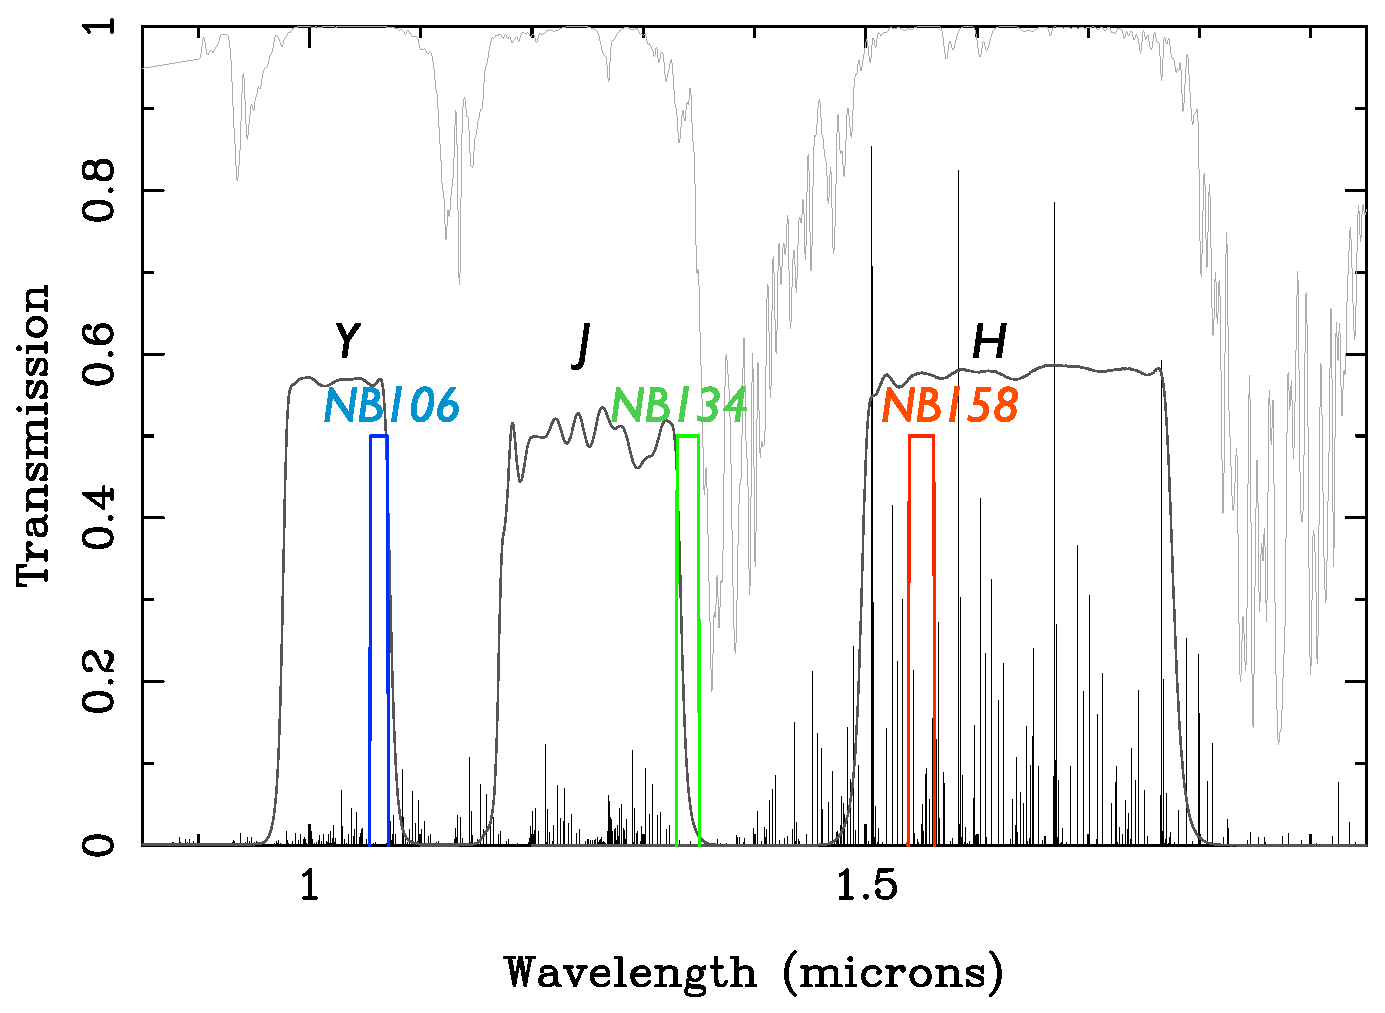
\includegraphics[width=80mm]{\thisdir figs/iwata_pg_filters_nbf01vd.eps}
}
\caption{
Transmission curves of NBFs considered. Transmission curves for $Y$,
 $J$, $H$-bands and the atomospheric transmission, and OH air glow
 strength (in arbitrary unit) are also shown.
}
\label{fig:iwata_filter_nbf}
\end{figure}

We assume read-out noise to be 10e$^-$ and dark current to be
0.01e$^-$/s. The plate scale is set to $0.117''$, which is the value of
MOIRCS.  Here we consider aperture photometry with diameter $\phi 0.5''$
and  $\phi 0.75''$ for observations with GLAO and those under natural
seeing, respectively\footnote{to-do: Check the fraction of point source
light falling within the apertures}.
We neglect the thermal emission from the telescope and
instruments\footnote{Although it may not be so large, we should include
thermal emission as one of noise components.}

For a comparison, we also calculated expected sensitivities of near-IR
space missions such as JWST/NIRCam and WISH. The telescope mirror sizes, 
plate scales, and sizes of field-of-view are summarized in
Table~\ref{tab:iwata_telescope_param}.

\begin{table}[!ht]
\begin{center}
\begin{tabular}{rccc}
\hline
 & Mirror size(m) & pixel scale (arcsec/pix) & FoV (arcsec$^2$) \\
\hline
Subaru & 8.2 & 0.117 & 28 / 177$^\ast$\\
JWST/NIRCam & 6.5 & 0.0317 & 9.68 \\
WISH & 1.5 & 0.155 & 840\\
\hline
\end{tabular}
\end{center}
\caption{
Mirror size, plate scle, and field-of-view for Subaru, JWST/NIRCam, and
 WISH. 
$\ast$: The field-of-view for the case under natural seeing is set to 28
 arcmin$^2$, while for the case with GLAO it is set to 177 arcmin$^2$
($\phi 15'$).
}
\label{tab:iwata_telescope_param}
\end{table}

In Fig.~\ref{fig:iwata_nbf_sens} and in Table~\ref{tab:iwata_nbf_sens} 
we summarize the expected 10$\sigma$ detection limit with on-source 10
hours exposures for Subaru under natural seeing, Subaru with GLAO,
JWST/NIRCam (N164), WISH(NB109, NB134, NB158).
JWST/NIRCam's NBF with the shortest central wavelength is
$\lambda=1.65\mu$m, and thus there is no NBF for NIRCam which can be
used to search for LAEs at $z<12$.\footnote{NIRISS has medium band
filters such as F140M and F158M, and has a capability of slitless
spectroscopy. See \href{http://www.stsci.edu/jwst/instruments/niriss}{http://www.stsci.edu/jwst/instruments/niriss}.}

\begin{figure}[!ht]
\centerline{
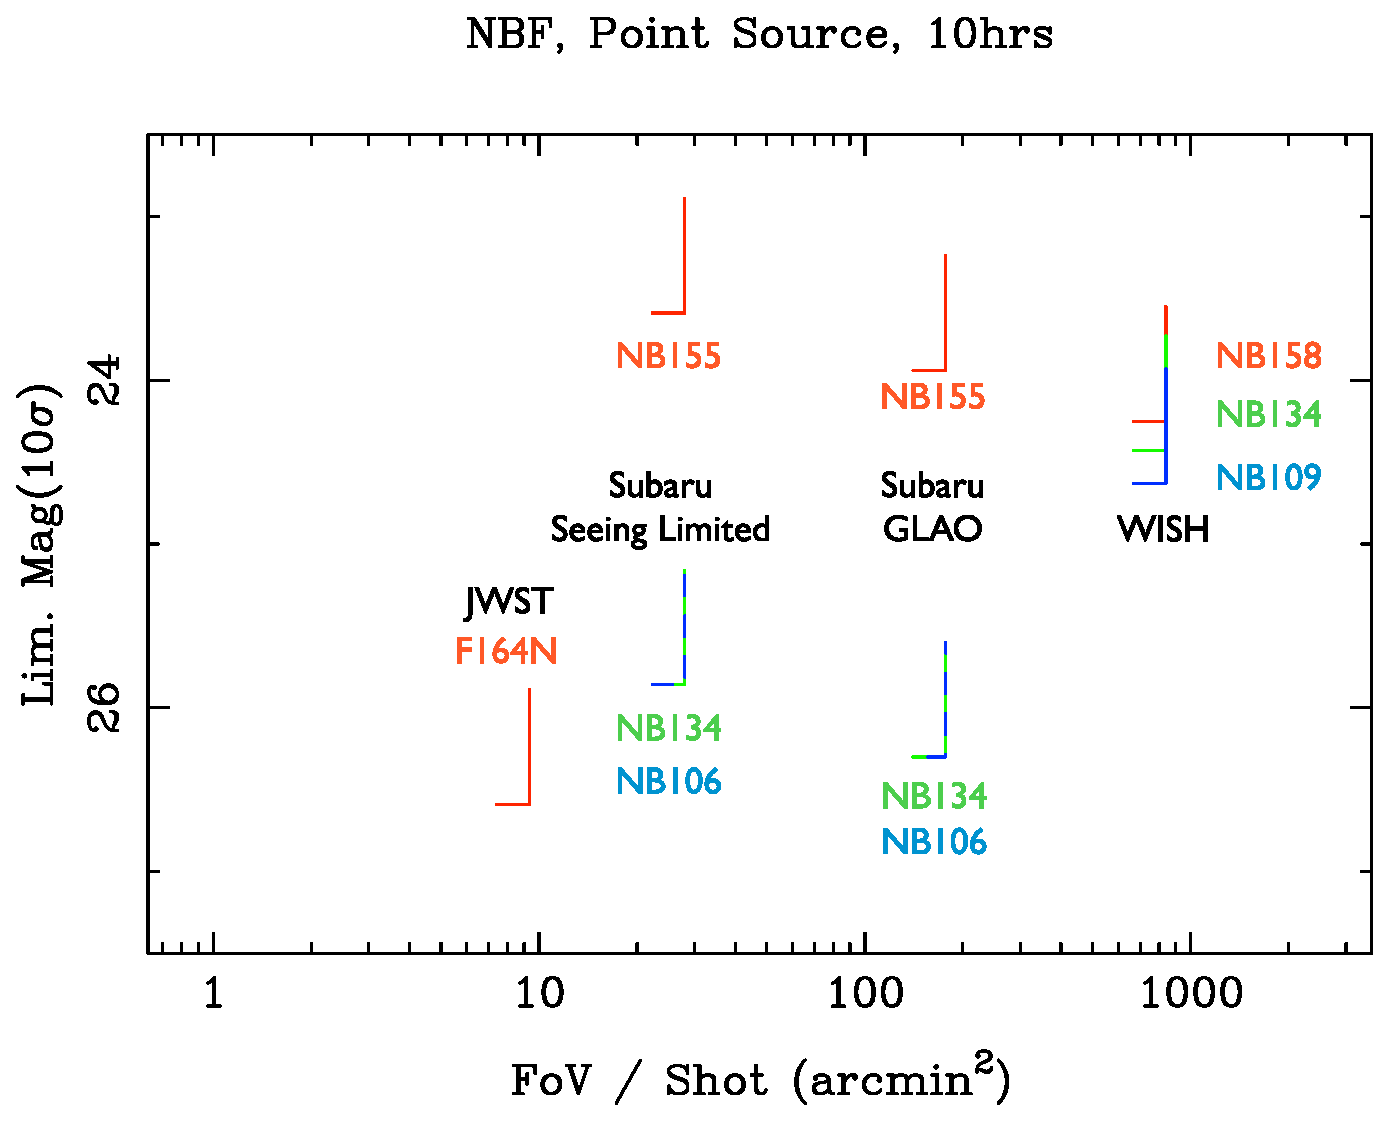
\includegraphics[width=80mm]{\thisdir figs/iwata_pg_fov08_nbf_vd.eps}
}
\caption{
Ten-$\sigma$ limiting magnitudes (in AB) with 10 hours of on-source
 exposure time for Subaru Telescope (natural seeing and GLAO),
 JWST/NIRCam, and WISH. See text for details.
}
\label{fig:iwata_nbf_sens}
\end{figure}

\begin{table}[!ht]
\begin{center}
\begin{tabular}{rccrrcc}
\hline
 & \multicolumn{2}{c}{Subaru Telescope} & \\
\cline{2-3}
 redshift & Natural seeing & GLAO & & redshift & WISH &
 JWST\\
\hline
 7.7 & 25.86 & 26.30 & & 8.0 & 24.63 & -- \\
 10.0 & 25.86 & 26.30 & & 10.0 & 24.43 & -- \\
 11.8 & 23.59 & 23.94 & & 12.5 & 24.25 & 26.69 \\
\hline
\end{tabular}
\end{center}
\caption{
Ten-$\sigma$ limiting magnitudes (in AB) with 10 hours of on-source
 exposure time for Subaru Telescope (natural seeing and GLAO),
 JWST/NIRCam, and WISH. See text for details.
}
\label{tab:iwata_nbf_sens}
\end{table}

\subsection{Expected Number of Detections}

Here we estimate the number of very high-z LAEs based on the expected
sensitivities described above and some assumptions on the evolution of
the LAE luminosity function (LF). 
We considered two cases for the evolution of LAE LF. 
One is the case that there is no evolution of LAE luminosity
function during the epoch considered, from the LAE LF at $z=6.5$
observationally obtained  by \citet{Kashikawa2011}.
Another case is that LAE LF evolves according to the prediction by the
semi-analytic model of galaxy evolution by \citet{Kobayashi2007,
Kobayashi2010} with updates on the model.
In \citet{Kashikawa2011} the authors argued that while the UV LF of LAEs
show little change from $z=5.7$ to $z=6.5$ there is a significant
decline of Ly$\alpha$ LF, and that could be due to the evolution of
neutral HI gas fraction between those epochs. If it is the case, even if
there is only small change in the number density of galaxies from 
$z\sim6$ to 12, the neutral fraction of IGM would be higher toward the
beginning to the cosmic reionization. So the case without the LAE LF
evolution should be the upper limit of the expected number of
detections. 
In Table~\ref{tab:iwata_lae_num1}, we show the number of detections per
single field-of-view with 10 hours on-source exposure time for the case
without LAE LF evolution from $z=6.5$.

\begin{table}[!ht]
\begin{center}
\begin{tabular}{rcccc}
\hline
 & \multicolumn{2}{c}{Subaru Telescope} & \\
\cline{2-3}
 redshift & Natural seeing & GLAO & WISH & JWST\\
\hline
 $\sim8$  & 0.5 & 8.3 & 0.2 & --\\
 $\sim10$ & 0.2 & 3.3 & 0.01 & -- \\
 $\sim12$ & 3e-8 & 8e-6 & 7e-4 & 0.3\\
\hline
\end{tabular}
\end{center}
\caption{
The expected number of detections per single field-of-view with 10 hours
 on-source exposure time. In this case it is assumed that there is no
 evolution of LAE Ly$\alpha$ LF from $z=6.5$ \citep{Kashikawa2011} to
 12. 
}
\label{tab:iwata_lae_num1}
\end{table}

In Table~\ref{tab:iwata_lae_num2} the expected numbers of LAE detections
based on the semi-analytic model by Kobayashi et al. are shown.
The number of detections become smaller compared to the case with no
evolution. If we make observations under natural seeing
conditions, it is almost impossible to detect $z\sim10$ galaxies. If we
use GLAO, however, we can expect $\sim0.4$ mag. sensitivity improvement
and larger field-of-view (in this calculation $\phi15'$ is
assumed). Those improvements open up the possibility of the detections
of LAE candidates at $z\sim10$, by executing deep surveys with $\sim10$
field-of-views. 
By detecting significant number of LAEs, we will be able to push the
observational constraints of neutral hydrogen gas fraction toward
$z\sim10$ by comparing the Ly$\alpha$ and UV LFs.
Moreover, these bright LAE candidates are excellent targets for
the follow-up spectroscopy by TMT (IRIS and IRMS) not only to confirm
their redshifts, but also to clarify the physical nature (size, mass,
amount of dust, star-formation rate, metallicity etc.) of these
galaxies in the very early stage of formation and evolution.

%\clearpage

\begin{table}[!htbp]
\begin{center}
\begin{tabular}{rccc}
\hline
 & \multicolumn{2}{c}{Subaru Telescope} & \\
\cline{2-3}
 redshift & Natural seeing & GLAO & JWST\\
\hline
 $\sim8$  & 0.4 & 3.9 & -- \\
 $\sim10$ & 0.03 & 0.5 & -- \\
 $\sim12$ & $\sim0$ & $\sim0$ &  0.003\\
\hline
\end{tabular}
\end{center}
\caption{
Same as Table~\ref{tab:iwata_lae_num1}, but in this case the evolution
 of Ly$\alpha$ LF based on the semi-analytic model of galaxy evolution
 by Kobayashi et al. is assumed.
}
\label{tab:iwata_lae_num2}
\end{table}


\subsection{Very Narrow Band Width Filters}

(TBW; Can the sensitivity be improved?)

\subsection{Proposed Observations}

In order to securely select candidates of LAEs, we need very deep
broad-band near-IR images to find objects with prominent emission
lines. 

\subsection{Synergy and Competitions}

\subsubsection{Synergy with TMT}

\subsubsection{Competitions with other facilities}

Instruments for 8--10m class telescopes.

ELT instruments.

Space-based projects.

\bibliographystyle{apj}
\bibliography{\thisdir nbf}
